\question (浙江大学,2000年)存储器的存取时间是指
\par\twoch{存储器的读出时间}{存储器的写入时间}{存储器进行连续读或连续写操作所允许的最短时间间隔}{\textcolor{red}{存储器进行一次读或写操作所需的平均时间}}
\begin{solution}D。
存取时间是指存储器进行一次读或写操作所需的平均时间。C选项是存取周期的定义。
\end{solution}
\question 设有一个1MB容量的存储器,字长为32位,按字节编址,那么地址寄存器和数据寄存器各为(
)位
\par\twoch{18、8}{18、32}{\textcolor{red}{20、8}}{20、32}
\begin{solution}C。 因为按字节编址,跟字长无关,那么数据寄存器也等于一个字节,即8位。
地址寄存器位数=log2(存储单元数)=log2(1MB/1B)=log2(1M)=log2(2\^{}20)=20。
【扩展】 如果这题改为,``按字编址''的话,那么答案为什么?
解法也是一样的,数据寄存器就需要能装下一个字,即32位(4B)。
地址寄存器位数=
log2(存储单元数)=log2(1MB/4B)=log2(256K)=log2(2\^{}18)=18。
\end{solution}
\question 由于CPU内部操作的速度较快,而CPU访问一次存储器的时间较长,因此机器周期通常由(
)来确定
\par\fourch{\textcolor{red}{主存中读取一个指令字的最短时间}}{主存中读取一个数据字的最长时间}{主存中写入一个数据字的平均时间}{主存中读取一个数据字的平均时间}
\begin{solution}A。
存储器的存取周期是指开始一次存取操作与下一次存取操作开始之前的最短时间间隔,通常从主存中读取一个指令字的最短时间就是存取周期。
\end{solution}
\question 假设基准程序A在某计算机上的运行时间为100s,其中90s为CPU时间,其余为I/O时间。若CPU速度提高50\%,I/O速度不变,则运行基准程序A所耗费的时间是(
)
\par\twoch{55s}{60s}{65s}{\textcolor{red}{70s}}
\begin{solution}首先,需要计算CPU速度提高之后的CPU时间,即90/(1+50\%)=60s,而I/O时间为10s是不变的,所以运行基准程序A所耗费的时间是60s+10s=70s。
\end{solution}
\question 程序P在机器M上的执行时间是20秒,编译优化后,P执行的指令数减少到原来的70\%,而CPI增加到原来的1.2倍,则P在M上的执行时间是(
)
\par\twoch{8.4秒}{11.7秒}{14.0秒}{\textcolor{red}{16.8秒}}
\begin{solution}程序的执行时间=CPI×指令数,指令数与CPI都和程序的执行时间成正比,优化编译之后,指令数下降到70\%,CPI增加到原来的1.2倍,则程序执行时间=1.2×CPI×指令数×70\%=1.2×20s×70\%=16.8s。
【总结】本题属于简单题,同类型的题源还有时钟频率和总线宽度的改变来讨论数据传输速率的问题;指令周期、机器周期、时钟周期的改变来讨论指令执行的时间问题,这类问题都都属于``此消彼长'',要明确各个参量之间的概念,计算不要出错。
\end{solution}
\question 32位和64位的个人计算机中,一个字节分别由( )位和( )位组成
\par\twoch{4、8}{\textcolor{red}{8、8}}{8、16}{16、32}
\begin{solution}不管个人计算机是多少位,一个字节都是由8位组成,这个是规定,是不可改变的。
\end{solution}
\question (中国科学院)用于科学计算的计算机中,标志系统性能的主要参数是( )
\par\twoch{主时钟频率}{主存容量}{\textcolor{red}{MFLOPS}}{MIPS}
\begin{solution}主时钟频率和主存容量越大,系统的性能越高,但不是标志性的参数。MFLOPS是每秒执行百万条浮点指令条数,是用来描述计算机浮点性能的,而用于科学计算的计算机主要就是看重浮点运算的性能,所以MFLOPS是衡量计算机系统的主要技术指标之一,故C选项正确。MIPS(Million
Instruction Per
Second)是每秒执行百万条指令条数,是用来描述一般的计算机系统性能的,并不同于专用于科学计算的评价标准。
\end{solution}
\question (华中师范大学,1997年)计算机操作的最小单位时间是( )
\par\twoch{\textcolor{red}{时钟周期}}{指令周期}{CPU周期}{中断周期}
\begin{solution}一个指令周期包含若干个CPU周期(机器周期),一个CPU周期包含若干个时钟周期。而中断周期为一个CPU周期,所以计算机操作的最小单位时间是时钟周期。
\end{solution}
\question 下列关于配备32位微处理器的计算机说法正确的是( )。
I.该机器的通用寄存器一般为32位 II.该机器的地址总线宽度为32位
III.该机器能支持64位操作系统
IV.一般来说,64位微处理器的性能比32位微处理器的高
\par\twoch{I和II}{I和III}{\textcolor{red}{I和IV}}{I、II和IV}
\begin{solution}微处理器的位数是指该CPU一次能够处理的数据长度,称为机器字长。通常机器字长等于通用寄存器的长度。故I正确。
地址总线宽度决定了CPU可以访问的物理地址空间,简单地说就是CPU到底能够使用多大容量的内存。而CPU位数与地址字长无关,更不用说地址总线宽度了。故II错误。
III错误,64位操作系统(通常向下兼容)需要64位CPU的支持,64位操作系统不仅是寻址范围增加到2\^{}64,同时要求机器字长64位。
IV正确,一般来说,计算机的字长越长,其性能越高。
\end{solution}
\question 已知计算机A的时钟频率为800MHz,假定某程序在计算机A上运行需要12s。现在硬件设计人员想设计计算机B,希望该程序在B上的运行时间能缩短为8s,使用新技术后可使B的时钟频率大幅度提高,但在B上运行该程序所需要的时钟周期数为在A上的1.5倍。那么,机器B的时钟频率至少应为(
)才能达到所希望的要求
\par\twoch{800MHz}{1.2GHz}{1.5GHz}{\textcolor{red}{1.8GHz}}
\begin{solution}设计算机i的时钟频率为Ri,时钟周期为Ti,时钟周期数为Ni。 ①
TA*NA=NA/RA=12s ② TB*NB=NB/RB=8s ③ NB=1.5NA ④ RA = 800MHz 解得RB=1.8GHZ
\end{solution}
\question 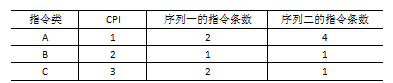
\includegraphics[width=4.09375in,height=0.86458in]{computerassets/f1ee365e16cc158b8b116a176c44b5d2.jpeg}

假定编译器对高级语言的某条语句可以编译生成两种不同的指令序列,A、B和C三类指令的CPI和执行两种不同序列所含的三类指令条数见上表。则以下结论错误的是(
~)。 I.序列一比序列二少1条指令 II.序列一的总时钟周期数比序列二多1个
III.序列一比序列二的执行速度快 IV.序列一的CPI比序列二的CPI大
\par\twoch{I和II}{I和III}{II和IV}{\textcolor{red}{III}}
\begin{solution}序列一的指令条数为5,序列二的指令条数为6,故I正确。 ~ ~ ~ ~
序列一需要总时钟周期数为1*2+2*1+3*2=10,序列二需要总时钟周期数为1*4+2*1+3*1=9,故II正确。
~ ~ ~ ~
由于序列一和序列二都是由高级语言的某条语句编译而成的,序列一花的时间长,则序列一的速度比序列二的速度慢,故III错误。
~ ~ ~ ~ 序列一的CPI为10/5=2,序列二的CPI为9/6,故IV正确。 ~ ~ ~
【总结】本题很容易误选B。因为考生很容易把CPI看成是执行速度的衡量。但此处的条件特殊,这两条不同的指令序列是为了实现同一条高级语言语句。也就是任务量是相等的,则花时间短的序列,执行速度就快。
\end{solution}
